%\documentclass{article} %[twocolumn] 
\documentclass[sagev]{sagej}

%\usepackage{algorithmic}
\usepackage{algorithm}
\usepackage{algorithmicx}
\usepackage{algpseudocode}
\usepackage{booktabs}
\usepackage{array}
\usepackage{graphicx}
\usepackage{amsmath}
\usepackage{amsfonts}
\usepackage{amssymb}
\usepackage{multirow}
\usepackage{url}

\setcounter{secnumdepth}{3} %Gives section numbers for cross referencing
\begin{document}

\runninghead{Wilson et al.}

\title{Robust, value-based sample size determination for clinical trials when nuisance parameters are unknown}

\author{Duncan T. Wilson\affilnum{1}}%,
%Rebecca E. A. Walwyn\affilnum{1}, 
%Richard Hooper\affilnum{2},
%Julia Brown\affilnum{1} and 
%Amanda J. Farrin\affilnum{1}}

\affiliation{\affilnum{1}Leeds Institute of Clinical Trials Research, University of Leeds, Leeds, UK} %\\
%\affilnum{2}Centre for Primary Care \& Public Health, Queen Mary University of London, London, UK}

\corrauth{Duncan T. Wilson, Clinical Trials Research Unit, Leeds Institute of Clinical Trials Research, University of Leeds, Leeds, LS2 9JT, UK}
\email{d.t.wilson@leeds.ac.uk}

\begin{abstract}
% 200 word limit (250 for YSM)

\textbf{Background:} The conventional approach to determining the sample size of a clinical trial is to choose the smallest value such that the power of the trial is above some nominal threshold, often 0.8 or 0.9. This sample size can be highly sensitive to nuisance parameters, such as the variance of a continuous primary outcome. Sample size re-estimation methods allow these parameters to be estimated at an interim analysis to allow the sample size to be adjusted accordingly. However, these methods do not formally account for the associated costs of increased sampling, and as a result can lead to incoherent decisions.

\textbf{Methods:} We present an alternative model for sample size determination which explicitly balances costs and benefits by introducing a value function to be maximised. We explore the implications of the model and argue it provides a better representation of sample size determination in practice than the conventional approach. We show the method is significantly less sensitive than the conventional approach to nuisance parameters, to the point where a fixed design with no interim sample size adjustment can be near-optimal for large regions of the nuisance parameter space. We propose a criterion for choosing an optimal fixed sample size, considering the range of nuisance parameter values for which the value of the fixed design is within a tolerable distance of the value of the best possible design.

\textbf{Results:} We illustrate our approach by applying it to two trial design problems: choosing the accrual and follow-up times for a parallel group trial comparing overall survival, where the median survival time in the control arm is unknown; and choosing the number of clusters in a cluster randomised trial with unknown variance components at both the individual and cluster levels.

\textbf{Conclusion:} Accounting for the costs of sampling when determining the sample size of a clinical trial,  we can find simple, fixed sample size designs which are highly robust to nuisance parameter uncertainty.
\end{abstract}

\keywords{Clinical trials, sample size, power, interim analysis}

\maketitle



\section{Introduction}\label{sec:intro}

Prepare and motivate.

Need to know:
- Standard SSD procedure (target difference, nuisance parameters, constrained optimisation)
- Implication of ignoring costs, especially as nuisance params vary
- The sample size samba, and how this accounts for cost informally
- Inability to do the samba in an SSR setting

Motivation:
- Conventional SSR leads to incoherent decisions, specifically to trials which are very inefficient in the sense that they are too large for the benefit they bring
- Need a new approach for SSD which can be appied in SSR coherently and transparently and which leads to more efficient trials






No real distinction between SSD and SSR, under the ideal case of perfect estimates. Question is just what sample size should be chosen for a given parameter value. We want a system for making that decision that's coherent. The current convention isn't, because it doesn't formally account for costs. It survives because people game the process, but this gaming relies on adjusting the target difference and we can't do that in the SSR setting. So, applying conventional SSR, we get interim decisions that do not cohere with the initial SSD decisions (e.g. deciding the same power is suddenly worth a lot more sampling).

We propose a simple method for accounting for cost and benefit through defining a value function and maximising it. We show how this leads to coherent decision making across nusiance parameter values, and therefore how it provides a basis for SSR. We then show that under our formulation fixed designs can be highly robust to nuisance parameter values and as such SSR can be avoided altogether, saving logisitcal headaches, money, keeping analyses simple (no multiple testing adjustments), and in many cases making the trial feasible (since the parameter can't be estimated with mch precision, e.g. hazard rate or ICC). We go on to suggest criteria for finding the best fixed design. We illustrate the general approach by applying to two examples.


\section{Body}

First, introduce some notation and describe conventional SSD and SSR more formally. We will consider a specific example, of a two-sample t-test with size $\alpha$ of a normally distributed outcome, with a common sd $\sigma$, balanced sample size $n$, and a difference in means to be detected of size $\mu$. We would like to minimise $n$ subject to the constraint $\beta(n, \mu, \sigma, \alpha) \leq \beta^*$, where $\beta(n | \mu, \sigma, \alpha)$ is the type II error rate for the trial with $n$, and $\beta^*$ is the constraint level, typically 0.1 or 0.2.

Generally, $\sigma$ is not known and is replaced by an estimate $\hat{\sigma}$, which may be from external data, internal pilot data, or expert judgement. The difference to be detected, $\mu$, should be the MCID.

We assume that all other things being equal, a higher powered trial is preferred to a lower powered trial; similarly, a trial of small sample size is preferred to a larger one. Under these assumptions, the constrained optimisation approach for choosing $n$ under different estimates $\hat{\sigma}$ will lead to varying choices of $n$ but a constant type II error rate of $\beta^*$. 

\subsection{Value-based design}

An alternative approach to SSD is to plot the power of the trial as a function of its sample size and to choose the point deemed to best balance cost (i.e. sample size) and benefit (i.e. power). To help describe this decision-making process formally, we can introduce a \emph{value} function $v(n, \beta): \mathbb{N} \times [0,1] \rightarrow \mathbb{R}$ which describes our preferences $\succ$ between all possible pairs of sample size and type II error. Specifically, $v$ is such that
$$
(n, \beta) \succ (n', \beta') \Leftrightarrow v(n, \beta) > v(n', \beta').
$$
Now, if we have a function $f(n)$ that returns the type II error rate obtained for any given choice of sample size (conditional on the remaining aspects of the trial design) then we can define our optimal sample size as
$$
n^* = {\arg\min}_{n \in \mathbb{N}} v(n, f(n)).
$$
We can safely assume that for any fixed $\beta$, $v_(n, \beta)$ as a function of $n$ will be strictly decreasing. We furthermore assume that it will also be linear, and that the gradient will be the same for all $\beta$. Together, these imply that the cost of increasing the sample size by some amount $\Delta$ is independent of the starting point $(n, \beta)$. Assuming the same holds when considering $v(n, \beta)$ as a function of $\beta$ for fixed $n$, the value function will be of the form
$$
v(n, \beta) = - (\beta + \lambda n)
$$
The optimal sample size can then be obtained by plotting the power curve for the problem at hand and finding the point where the tangent has gradient of $\lambda$. For example, consider a two sample t-test and a value function with $\lambda = 0.025$. Power of the test is that to detect an MCID of 1, under three estimates of the outcome standard deviation $\sigma = 0.7, 1, 1.3$. Each of the three power curves are plotted in Figure \ref{fig:ex1_3tangents}, along with the corresponding sample sizes resulting from maximising the value function. We see that the optimal sample sizes for $\sigma = 0.7, 1, 1.3$ are $n = 12, 17, 18$ with powers 0.92, 0.81, 0.61 respectively.

\begin{figure}
\centering
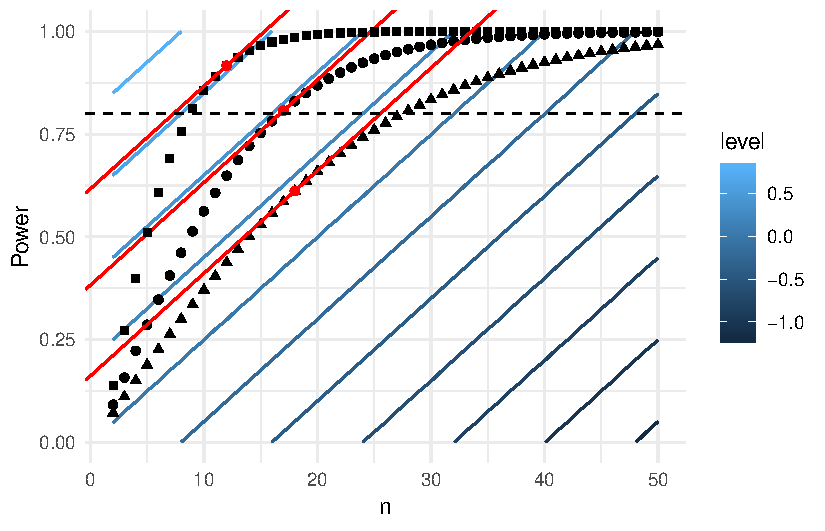
\includegraphics[scale=0.8]{./figures/ex1_3tangents}
\caption{.}
\label{fig:ex1_3tangents}
\end{figure}

\subsection{Sample size samba}

The value-based model for SSD initially appears to be completely incompatible with conventional SSD methods, leading as it does to powers substantially above or below the usual nominal values of 0.8 and 0.9. On reflection, however, it may actually be a superior descriptive model than the constrained method when we account for the common practice of `gaming' SSD calculations by adjusting the difference to be detected until a `feasible' sample size results - the so-called `sample size samba'. For example, suppose the true MCID is $\mu = 1$. An initial guess of $\hat{\sigma} = 1$ gives a sample size of $n = 17$ to achieve 80\% power. If we were told our initial estimate of $\sigma$ was incorrect and that actually $\sigma = 1.3$, the constrained method tells us to revise the sample size to $n = 27$. We consider this to be infeasible, and pretend that our MCID is actually $\delta = 1.23$. Then, $n = 18$ will give us 80\% power for this new target difference, but 61\% for the true MCID. Using the value-based method we would arrive at the same design of $n = 18$, but through an altogether more transparent route.

\subsection{Re-estimation}

In the fixed design setting, with a single estimate $\hat{\sigma}$, the sample size samba may allow sampling costs to be considered implicitly and thus arrive at the same design choice as would be obtained using the value method. It is, however, an opaque approach, and when the true MCID has been decided upon and published it will not be possible at all. In the re-estimation setting, where we expect at least one further estimate $\hat{\sigma}_2$ to be obtained, it is not possible since the MCID will have already been declared. Following the conventional approach will then force us to accept potentially absurb inflations to the sample size to maintain the same power, or to stop recruiting to the trial and just analyse the data obtained by that point. If re-estimating using the value-based method, any increases in the sample size will be bounded.

\subsection{Fixed designs}

As illustrated above, the value-based approach leads to sample size choices which are considerably less sensitive to the nuisance parameter. This lack of sensitivity means that, in some cases, the benefits gained through adjusting the sample size after obtaining an interim estimate can be limited, and so it may be preferable to use a fixed design and avoid the logistical and statistical complications that an interim analysis brings. We now consider a possible optimality criterion which could be used to choose such a fixed design.

Denote the fixed design sample size by $n^*$, and the optimal (value maximising) sample size as a function of the nuisance parameter by $n(\sigma)$. Then, for any $\sigma$, we can calculate the difference in value between the fixed and optimal designs:
$$
\delta(\sigma | n^*) = v(n(\sigma)) - v(n^*).
$$
We can then choose a fixed design by maximising the area of nuisance parameter space $\Sigma$ over which the discrepancy $\delta(\sigma | n^*)$ is within some tolerable amount, $\delta^*$. That is, we solve
$$
\max_{n^*} \int_{\Sigma} I[\delta(\sigma | n^*) \leq \delta^*] d\sigma.
$$

An alternative criterion could be to minimise than maximum discrepancy over some area of interest in the nuisance parameter space.


\subsection{Known nuisance parameters}

Normative model is also descriptive, justifying the `sample size samba'.

\subsection{Unknown nuisance parameters}



\section{Examples}

\subsection{Cluster RCT}

Consider a cluster RCT comparing two groups based on the mean of their continuous primary outcomes. In each arm we need to choose the number of clusters $k$ and the number of participants $n$. The MCID is $\mu = 0.3$, and the unknown nuisance parameters are the total variance $\sigma_T^2 = \sigma_B^2 + \sigma_W^2$ and the ICC $\rho = \sigma_B^2/\sigma_T^2$.

To determine the parameter values for the value function, we take an initial guess for the parameter values at $\sigma_T^2 = 1$ and $\rho = 0.05$ and plot the power of the trial as a function of $n$ for various levels of $k$. This is shown in Figure \ref{fig:cluster_pow}.

\begin{figure}
\centering
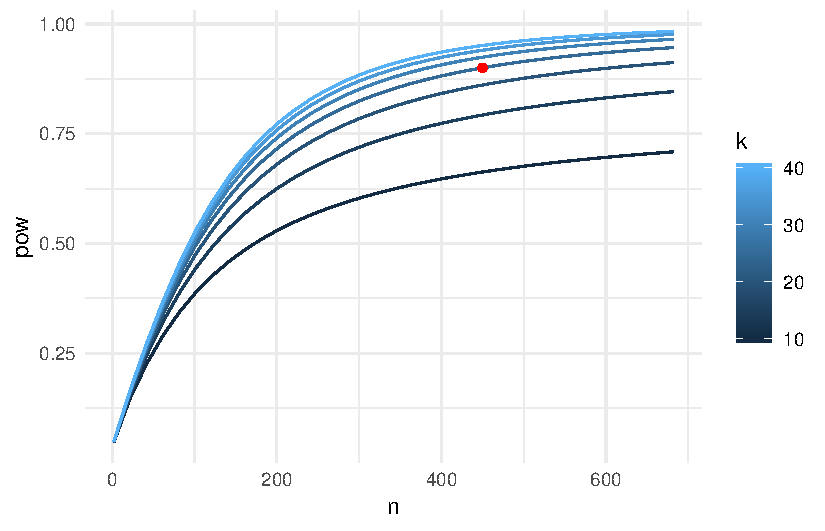
\includegraphics[scale=0.8]{./figures/cluster_pow}
\caption{.}
\label{fig:cluster_pow}
\end{figure}

From the power curves, we decide that the point $k=25, n=450$ offers the best trade-offs between sampling at each level and power. We then calculate the corresponding value function parameter, $\lambda = (0.006026021, 0.000324420)$. Calculating the value of optimal designs for a range of nuisance parameter values, we can plot the discrepancies between these and the value of the original fixed design as shown in Figure \ref{fig:cluster_disc}.

\begin{figure}
\centering
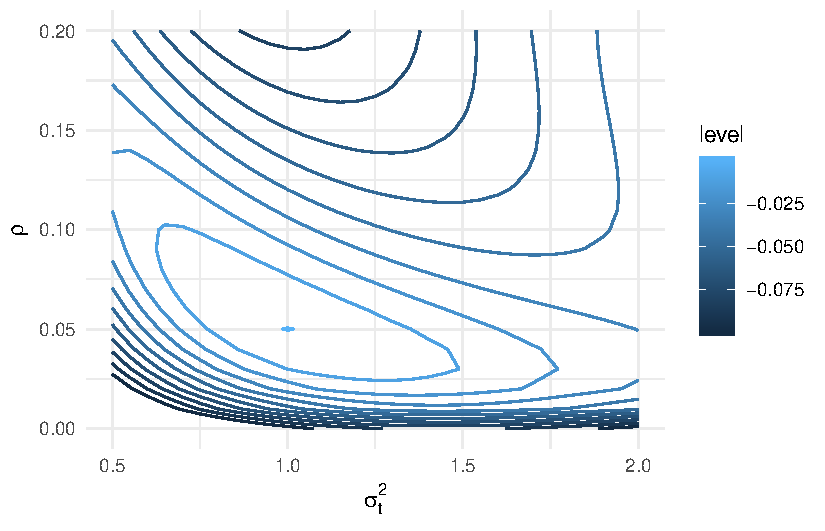
\includegraphics[scale=0.8]{./figures/cluster_disc}
\caption{.}
\label{fig:cluster_disc}
\end{figure}

\subsection{Survival}

\section{Discussion}

Ethics of underpowered and overpowered studies; the threshold myth.

\cite{Schulz2005} - Sample size calculations in randomised trials: mandatory and mystical

\cite{Halpern2002} - The continuing unethical conduct of underpowered clinical trials

\cite{Lilford2002} - The Ethics of Underpowered Clinical Trials

\cite{Bacchetti2005a} - Ethics and sample size

\cite{Bacchetti2005} - Bacchetti et al. Respond to ``Ethics and sample size - Another view''

\cite{Norman2012} - Sample size calculations: should the emperor's clothes be off the peg or made to measure?

\cite{Edwards1997} - Why "underpowered" trials are not necessarily unethical

\cite{Girling2007} - Sample-size calculations for trials that inform individual treatment decisions: a 'true-choice' approach

\cite{Claxton1999} - The irrelevance of inference: a decision-making approach to the stochastic evaluation of health care technologies

\cite{Grayling2018} - Blinded and unblinded sample size reestimation procedures for stepped-wedge cluster randomized trial

\cite{Altman1980} - Statistics And Ethics In Medical Research: III How Large A Sample?

\cite{DeMartini2010} - Conservative Sample Size Estimation in Nonparametrics

\begin{acks}
Acknowledgements.
\end{acks}

\begin{dci}
The Authors declare that there is no conflict of interest.
\end{dci}

\begin{funding}
This work was supported by the Medical Research Council [grant number xxx].
\end{funding}

\bibliographystyle{SageV}
\bibliography{C:/Users/meddwilb/Documents/Literature/Databases/DTWrefs}

\end{document}
